\chapter{Operating-System Structures}

OS has the task of interconnecting HW and SW. It provides function that are helpful to the user: system call, services, user interface, I/O, file system, network interface, error detection, resource allocation, security and so on.

\begin{figure}[htbp]
    \centering
    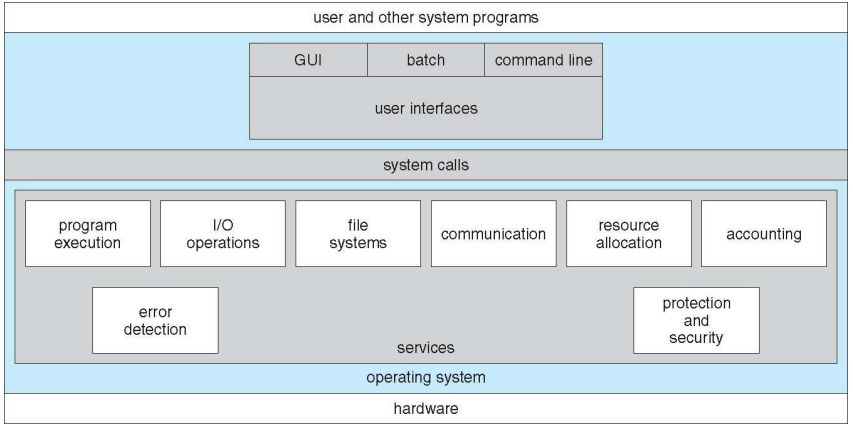
\includegraphics[width=0.7\linewidth]{img/SO.png}
\end{figure}

\section{Operating System Services }

\subsection{(G)UI}

CLI or command line interface allows detect command entry. The basic CLI in windows is Command Prompt, also known as cmd.exe or cmd. CLI existing in each OS (Windows, Max, Linux and Solaris etc.).

Nowadays the UI is more user-friendly tanks the graphics, programme icons, button, directory, files etc. Even if  OS now include GUI, they also have the old CLI.


\newpage
\section{System Calls}
System Calls are typically written in high-level language (C, C++). Most libraries include specific functions that allows programmers to call the operating system call. 

Most common API are:
\begin{itemize}
    \item Win32 API for Windows
    \item POSIX API for POSIX-based systems (UNIX, Linux and Max OS X)
    \item Java API for the Java virtual machine (JVM)
\end{itemize}


Example of System call to copy the contents of one file to another file:


\begin{figure}[htbp]
    \centering
    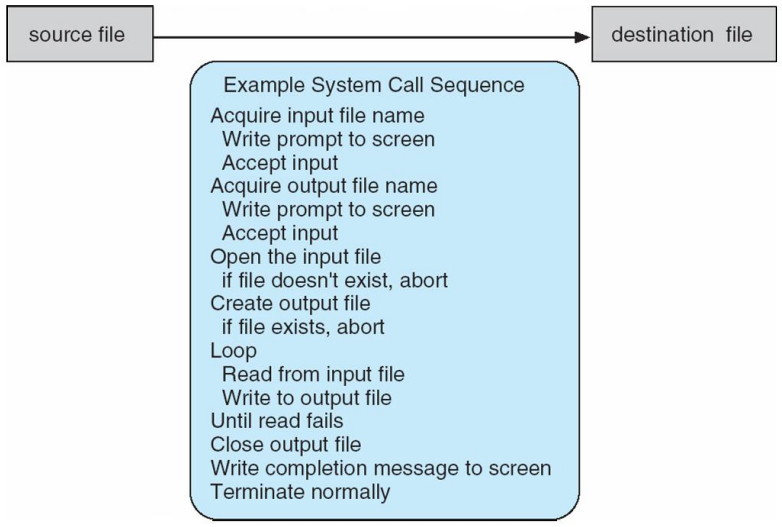
\includegraphics[width=0.6\linewidth]{img/image.png}    
    
\end{figure}

Example of API:

% \begin{lstlisting}[language=c]
% #include<unistd.h>

% ssize_t read(int fd, void *buf, size_t count)

% \end{lstlisting}

\begin{codeInC}
#include<unistd.h>
ssize_t read(int fd, void *buf, size_t count)
\end{codeInC}

\paragraph{}

But why do not programmers call the operating system call themselves instead of calling the library function?


The answar is \textbf{portability}. Programmer do not care about the implementation and the name of OS-call. So we shift the problems to the libraries. Different libraries (for different OS) implement the right system call.

Another answar is \textbf{Error}. If i call an OS-call with different type, e.g. an  integer instead of character parameter, I bother the OS and the CPU because OS throw an error.
Although if I call a function inside the program language library, it checks if all is right and forwards the request to the OS. 

\newpage
\subsubsection{API and OS Security}

\begin{figure}[htbp]
    \centering
    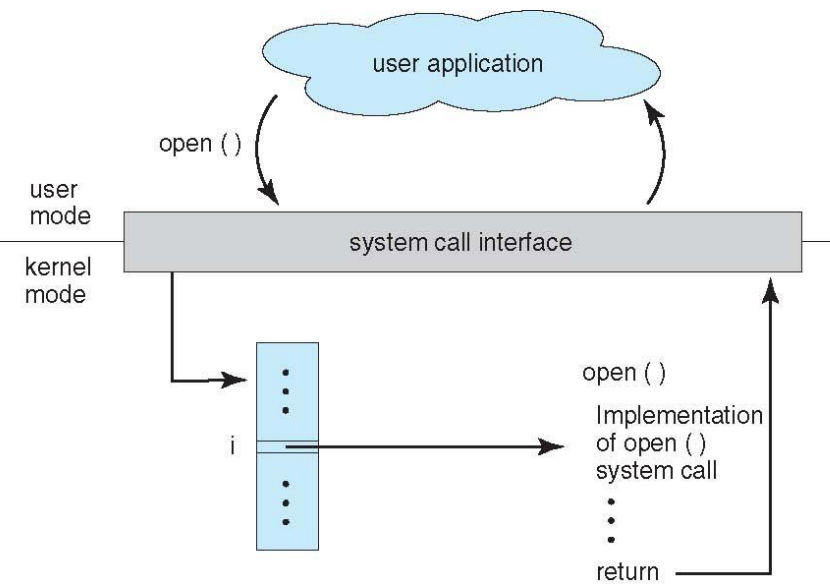
\includegraphics[width=0.6\linewidth]{img/API.png}
\end{figure}


\subsection{System call parameter passing}

There are three way to pass the parameters to OS-call:
\paragraph{}
-- The \textbf{firth}, the easiest way, is to copy all parameters into the registers but not always this method works. Normally the registers are less then the parameters.

\paragraph{}
-- The \textbf{second} way is to copy all parameters into a table or block and storing it in the ram and loading on register address of the cell where parameters are located.

This approach is used by Linux and Solaris OS.

\paragraph{}
-- The \textbf{last} approach is: Parameters placed, or pushed, onto the stack by the program
and popped off the stack by the operating system.


\begin{figure}[htbp]
    \centering
    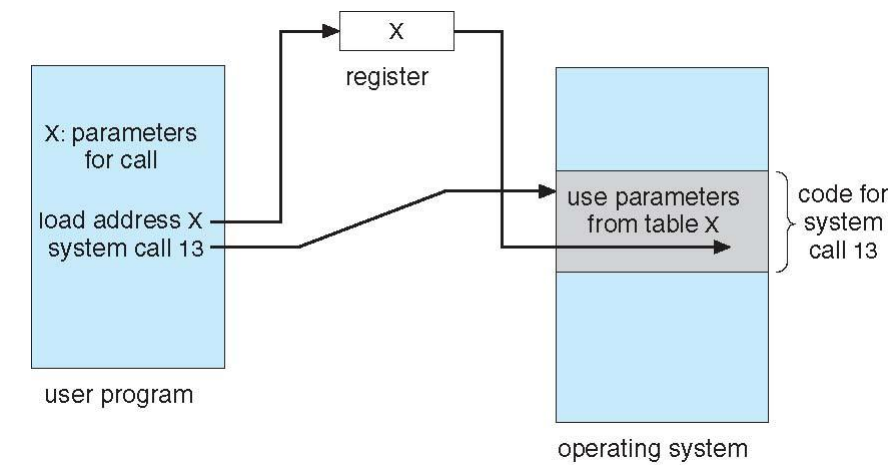
\includegraphics[width=0.6\linewidth]{img/params.png}
\end{figure}


\newpage
\subsection{Types of system call}

\begin{itemize} 

\item Process control
     \begin{itemize} 
        \item create process, terminate process
        \item end, abort
        \item load, execute
        \item wait for time
        \item wait event, signal event        
     \end{itemize}
     
\item File management
     \begin{itemize} 
        \item open, close
        \item create file, delete file
        \item read, write, append      
     \end{itemize}

\item Device management
     \begin{itemize} 
        \item read, write, reposition
        \item request device, release device
        \item logically attach or detach devices   
     \end{itemize}

\item Information maintenance
     \begin{itemize} 
        \item get time or date, set time or date
        \item get system data, set system data
     \end{itemize}

\item Communications
     \begin{itemize} 
        \item create, delete communication connection
        \item Shared-memory
        \item transfer status information
     \end{itemize}

\item Protection
     \begin{itemize} 
        \item Control access to resources
        \item Get and set permissions
        \item Allow and deny user access
     \end{itemize}
\end{itemize}



\begin{figure}[htbp]
    \begin{minipage}[htbp]{0.5\textwidth}
        \centering
        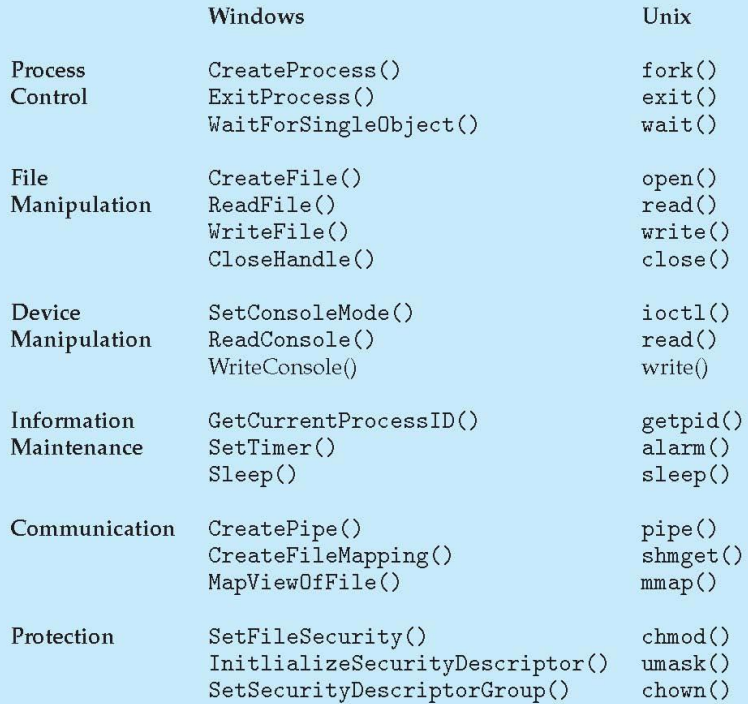
\includegraphics[width=0.9\linewidth]{img/SC.png}
    \caption{Windows and Unix System Call}
    \end{minipage}
    \begin{minipage}[htbp]{0.5\textwidth}
    \centering

    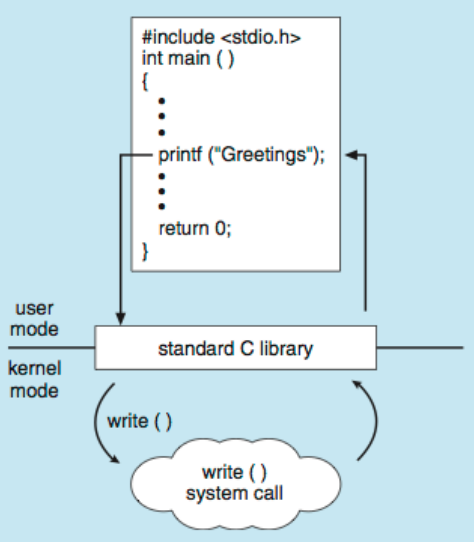
\includegraphics[width=0.8\linewidth]{img/print.png}
    \caption{Standard C library}       
    \end{minipage}
\end{figure}


\newpage
\subsection{MS-DOS}

The first OS (1982-2000) can run only single program, to open new program user must reload shell.

\subsection{FreeBSD}

First multitasking OS. Shell can open more then one program at the same time.

\section{Operating System Design and Implementation}
There aren't the best way to create an OS, it depends to different things:

\begin{itemize}
    \item HW
    \item SW
    \item Updating
    \item Usability...
\end{itemize}

\begin{itemize}
    \item \textbf{User Goals: }easy to learn, reliable, safe and fast.
    \item \textbf{System goals: }operating system should be easy to design, implement, and maintain, as well as flexible, reliable, error-free, and efficient
\end{itemize}

\paragraph{}
Some of this things conflict with the each other. GUI is more user-friendly but is more complex to implement GUI instead of CLI.

Some important principle to separate:

\begin{itemize}
    \item Policy: What will be done? policies decide what will be done

    \item Mechanism: How to do it? Mechanisms determine how to do something
\end{itemize}

\textbf{Example: }
\begin{itemize}
    \item[] Problem: exercising many processes
    \item[] Mechanism: Scheduling
    \item[] Policy: processes that use disk first, processes from a given user first, daemons first
\end{itemize}

\newpage
\section{Different kernel implementation}
There are different approach to implement the kernel in modern operating system; let's have a look of most of them.

\subsection{Monolithic Kernel - UNIX}
Original UNIX Kernel had a monolithic kernel structure splitted in two parts:

\begin{itemize}
    \item System programs
    \item The Kernel: Consists of everything below the OS-call interface and above the physical HW. Also it provides file system, other OS-function.
\end{itemize}

-- The pro of this approach: fast and energy efficient.

-- The cons: is not modulable, thus even small update requires recompilation from scratch and re-installation; no option to customize
\paragraph{}
This approach is the most used for OS kernel: linux use it and also android.




\subsection{Layered Approach}
OS is divided into a number of layers each with specific task built on top of lower layers. 

The \textbf{bottom} layer is the HW. The highest is the user interface.



This is more modular than monolithic approach. If you want to add or update some function in N-layer you just do it and recompile only N-layer and not all kernel.

Another aspect of this method, that remember TCP/IP stack, is that each level can only communicate with the lower level. 

\begin{figure}[htbp]
    \centering
    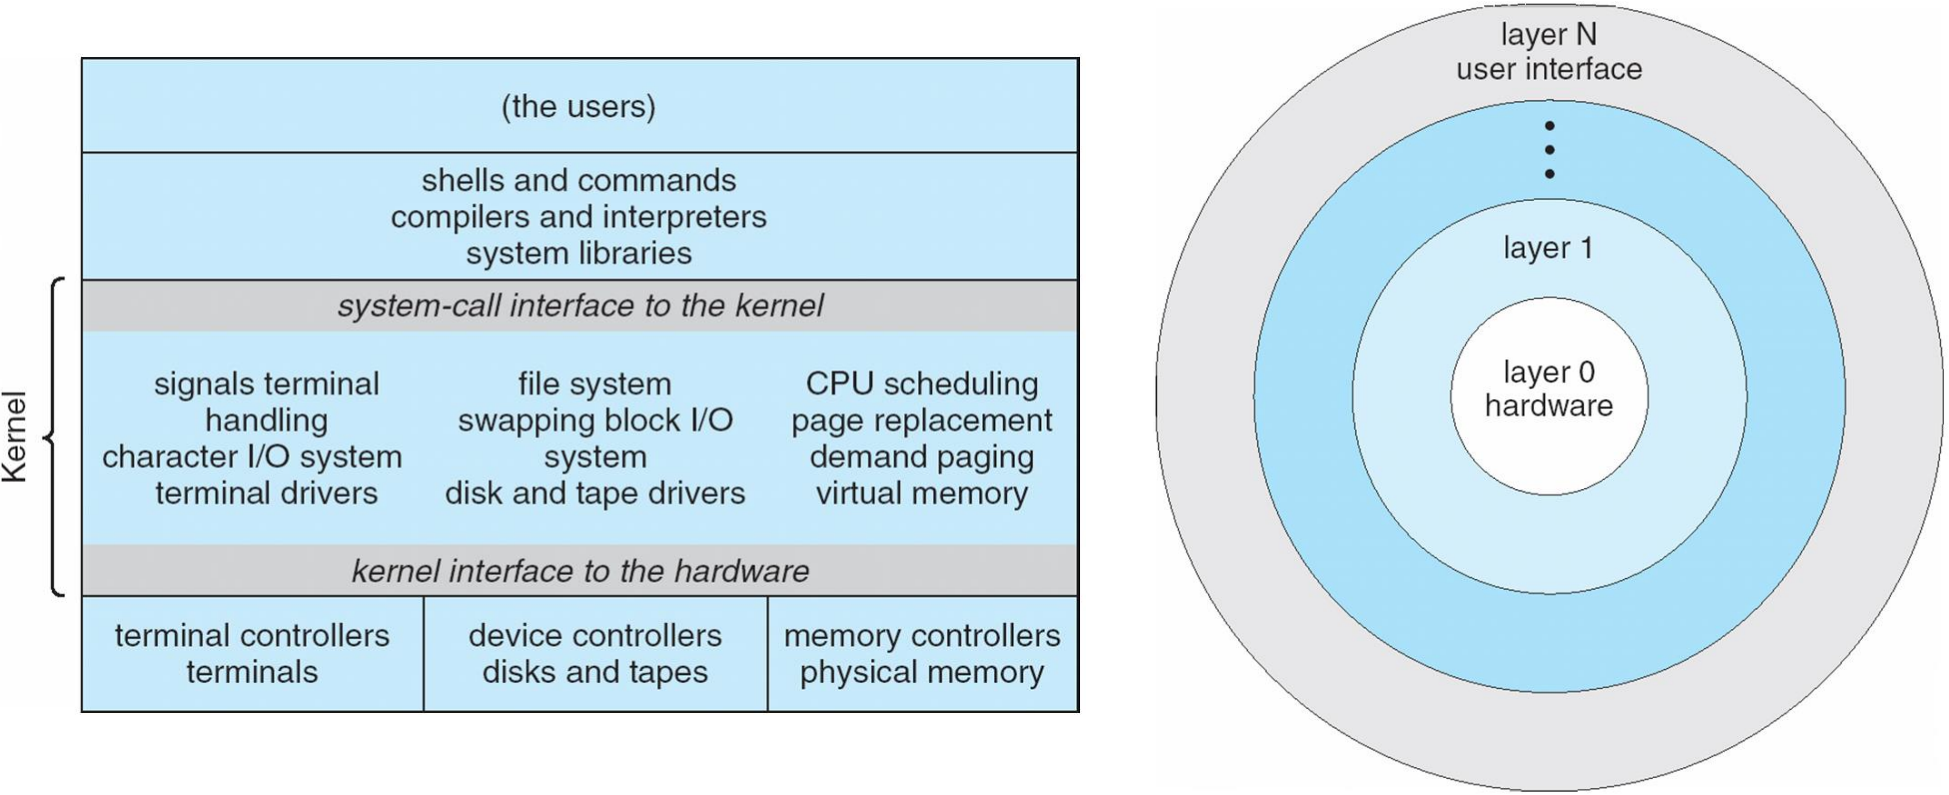
\includegraphics[width=0.85\linewidth]{img/kernel_mono_layer.png}
    \caption{Monolithic kernel left, Layered kernel right}
    
\end{figure}


\newpage
\subsection{MicroKernel System Structure}
MicroKernel is the tecnique that allow the most modular kernel. \textbf{Mach} is a particular example of microkernel, Max OS X kernel (Darwind) is based on Mach.

Obviously ther are pro and cons:
\paragraph{Pro:}
Easy to extend (best \textbf{modulability}); \textbf{portability} from OS to another with new architectures; \textbf{reliable} less cose running in kernel mode; \textbf{secure} malicious users process cant damage others.


\paragraph{Cons:}
Worst performance, lots of overhead is not direct communication because app must send a message to basic function of kernel.

\begin{figure}[htbp]
    \centering
    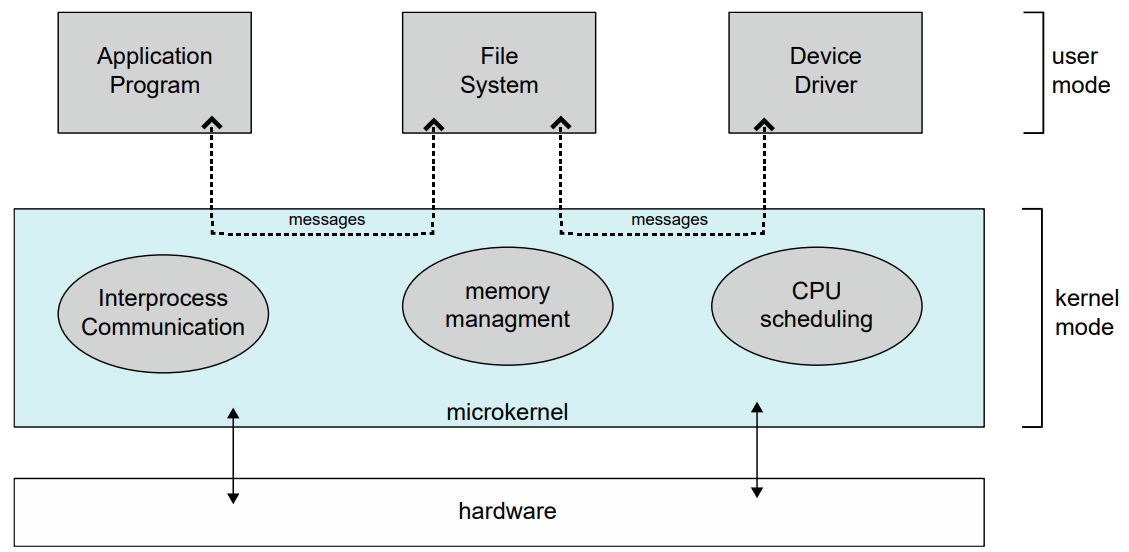
\includegraphics[width=0.6\linewidth]{img/microKer.png}
    \caption{micro kernel}
\end{figure}

\subsection{Solaris Modular Approach}
Solaris is OS used in business and/or commercial area that heavily use Oracle applications (Oracle DB, Java).

\subsection{Hybrid System}
Modern OS is a blended of monolithic, layer and microkernel features.
For example Windows is mostly monolithic but also it use microkernel structure. Also Mac OS X and Linux have a mix of different kernel structure.


\begin{figure}[htbp]
    \centering
    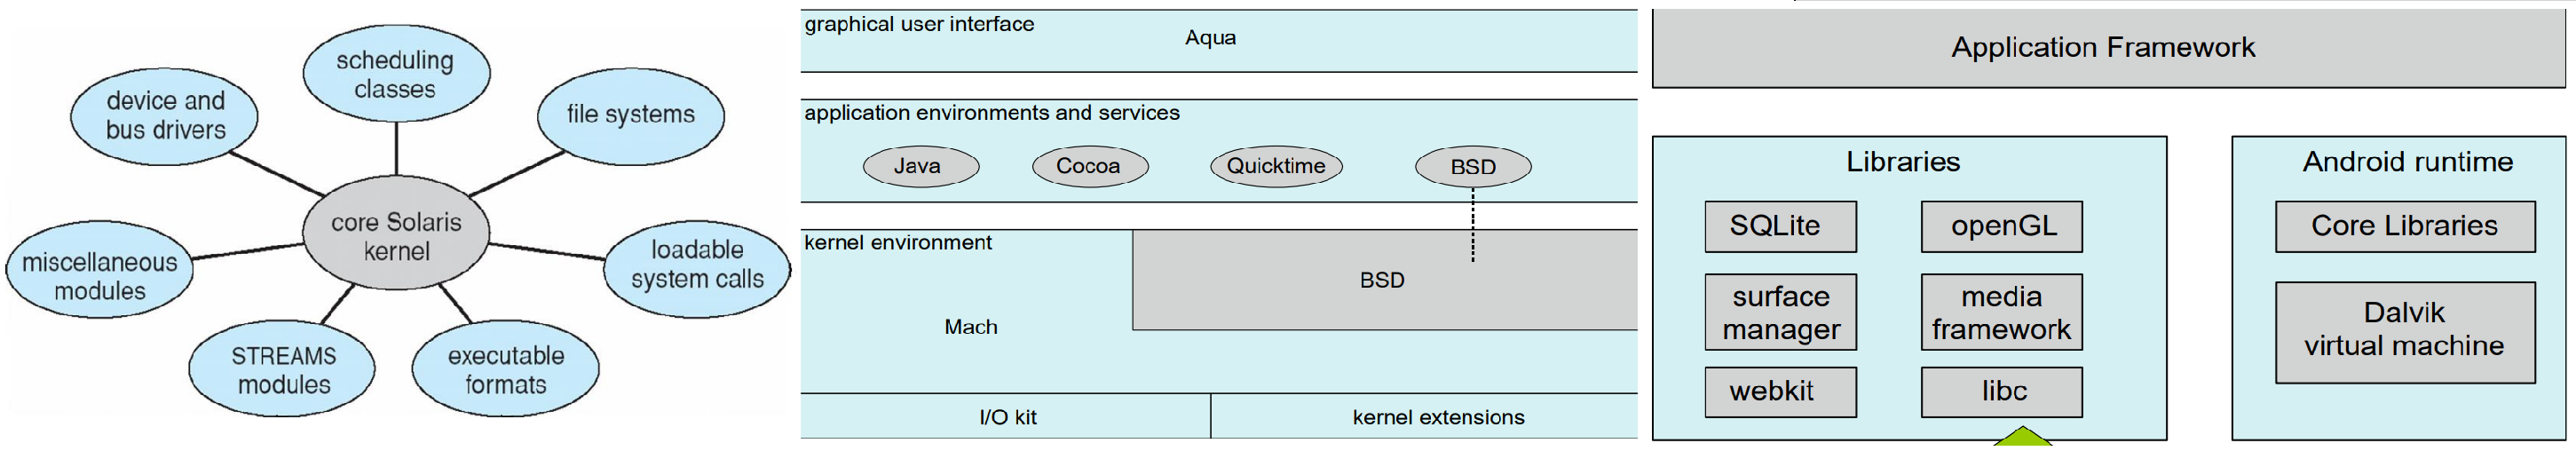
\includegraphics[width=1\linewidth]{img/kernel_3.png}
    \caption{Solaris left; Mac OS X center; Android right}
    
\end{figure}